\lstinputlisting[language=bash,basicstyle=\small]{python_codes/fieldstone_13/keywords.ascii}

\begin{center}
Code at \url{https://github.com/cedrict/fieldstone/tree/master/python_codes/fieldstone_13}
\end{center}

{\sl This fieldstone was developed in collaboration with BSc student Eric Hoogen}. 
\index{contributors}{E. Hoogen}

\par\noindent\rule{\textwidth}{0.4pt}

%%%%%%%%%%%%%%%%%%%%%%%%%%%%%%%%%%%%%%%%%%%%%%%%%%%%%%%%%%%%%%%%%%%%%%%%%%%%%%%%%%%%%%%%%%%%


After the initial setup of the grid, markers can then be generated and placed in the domain. One could simply randomly generate 
the marker positions in the whole domain but unless a {\it very} large number of markers is used, the chance that an element does 
not contain any marker exists and this will prove problematic. In order to get a better control over the markers spatial distribution, 
one usually generates the marker per element, so that the total number of markers in the domain is the product of the number of 
elements times the user-chosen initial number of markers per element. 

Our next concern is how to actually place the markers inside an element. Two methods come to mind: on a regular grid, or in a random manner, 
as shown on the following figure:

\begin{center}
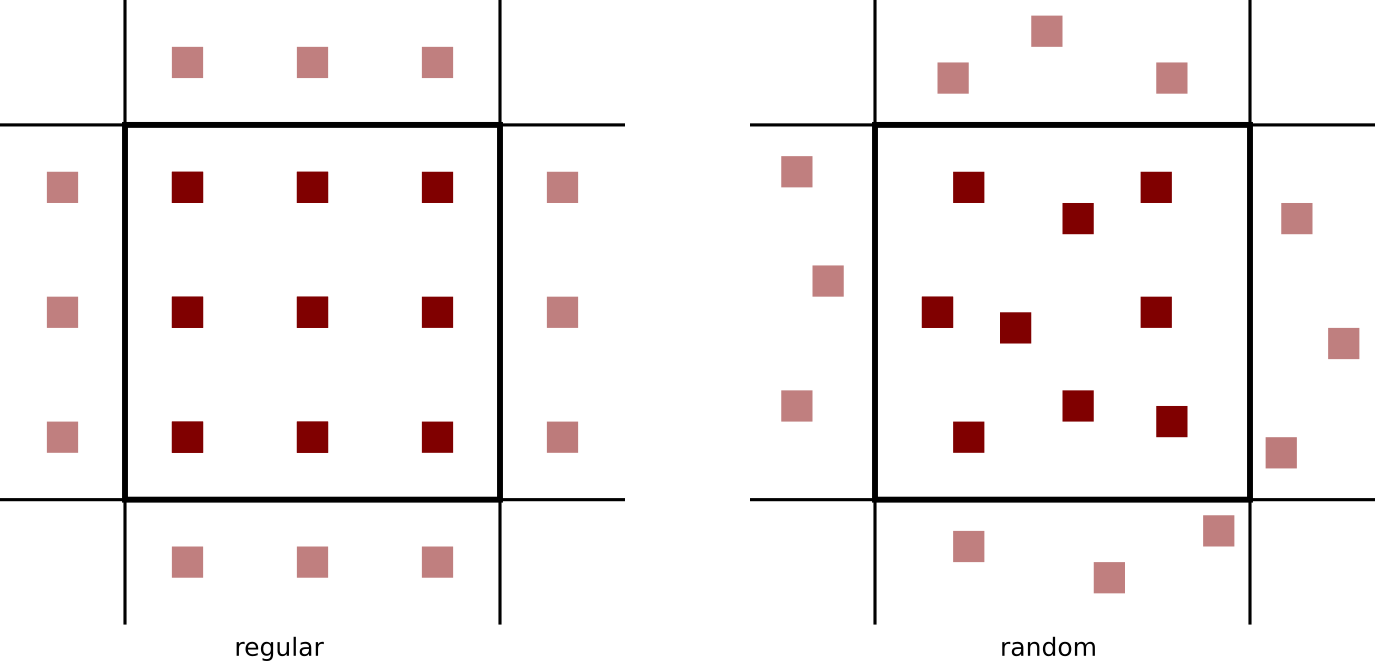
\includegraphics[width=8cm]{python_codes/fieldstone_13/markers} 
\end{center}

In both cases we make use of the basis shape functions: we generate the positions of the markers (random or regular) in the reference
element first ($r_{im},s_{im}$), and then map those out to the real element as follows:
\begin{equation}
x_{im}=\sum_i^m N_i(r_{im},s_{im}) x_i
\quad\quad\quad\quad
y_{im}=\sum_i^m N_i(r_{im},s_{im}) y_i
\end{equation}
where $x_i,y_i$ are the coordinates of the vertices of the element.

A third option consists in the use of the so-called Poisson-disc sampling which 
produces points that are tightly-packed, but no closer to each other than 
a specified minimum distance, resulting in a more natural pattern 
\footnote{https://en.wikipedia.org/wiki/Supersampling}. Note that 
the Poisson-disc algorithm fills the whole domain at once, not element after element.

{\color{red} say smthg about avrg dist}  

{\color{red} insert here theory and link about Poisson disc }

\begin{center}
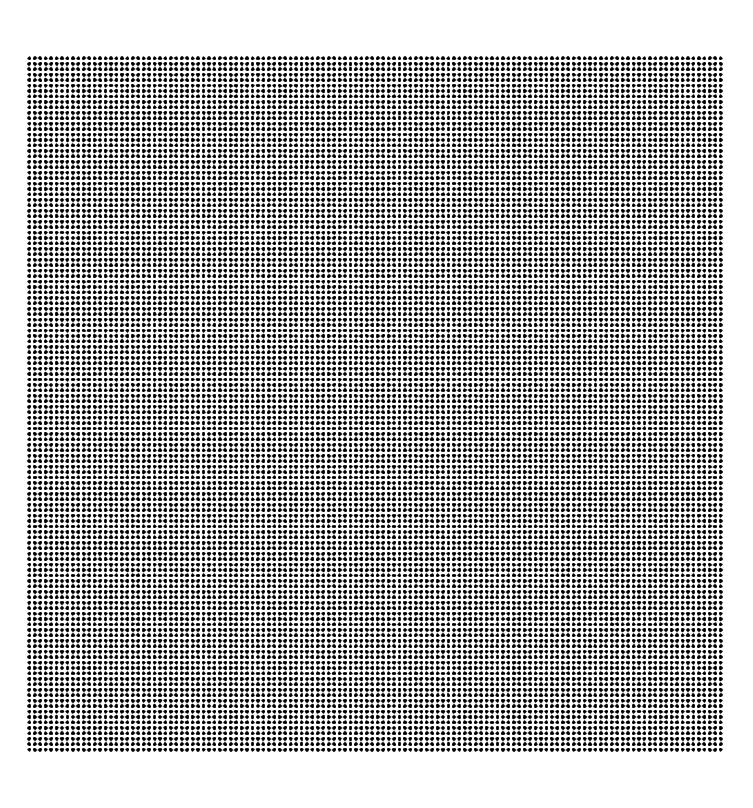
\includegraphics[width=5.134cm]{python_codes/fieldstone_13/images/markers_reg} 
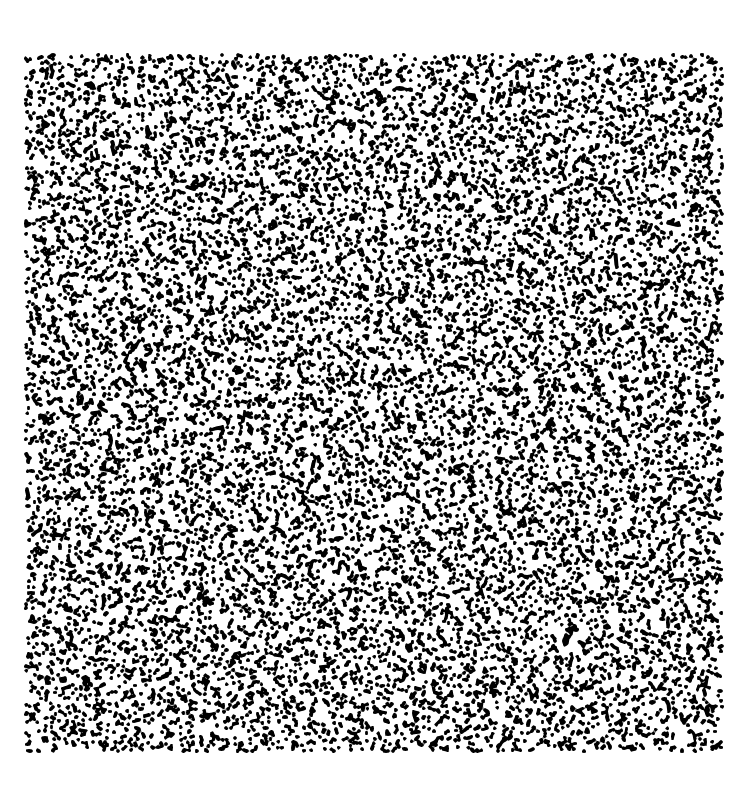
\includegraphics[width=5.134cm]{python_codes/fieldstone_13/images/markers_rand} 
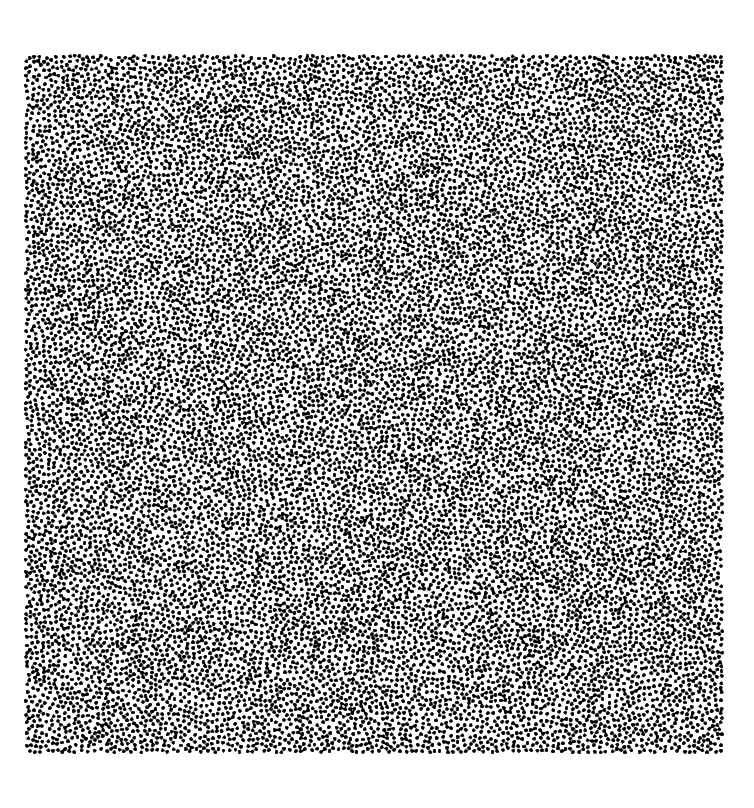
\includegraphics[width=5.134cm]{python_codes/fieldstone_13/images/markers_pd} \\
{\small Left: regular distribution, middle: random, right: Poisson disc.\\
 16384 markers (32x32 grid, 16 markers per element).}
\end{center}



When using {\it active} markers, one is faced with the problem of transferring the properties they carry to the mesh on which the PDEs are to be solved. 
As we have seen, building the FE matrix involves a loop over all elements, so one simple approach consists of assigning each element a single property
computed as the average of the values carried by the markers in that element. 
Often in colloquial language "average" refers to the arithmetic mean: 
\begin{equation}
\langle \phi \rangle_{am}=\frac{1}{n} \sum_k^n \phi_i 
\end{equation}
where $<\phi>_{am}$ is the arithmetic average of the $n$ numbers $\phi_i$. 
However, in mathematics other means are commonly used, such as the geometric mean: 
\begin{equation}
\langle \phi \rangle_{gm}=\left( \prod_i^n \phi_i \right)
\end{equation}
PROBLEM with this formula!!!!
and the harmonic mean: 
\begin{equation}
\langle \phi \rangle_{hm}=\left( \frac{1}{n}\sum_i^n \frac{1}{\phi_i} \right)^{-1}
\end{equation}
Furthermore, there is a well known inequality for any set of positive numbers,
\begin{equation}
\langle \phi \rangle_{am}\quad  \geq \quad
\langle \phi \rangle_{gm}\quad  \geq \quad
\langle \phi \rangle_{hm} 
\end{equation}
which will prove to be important later on. 

Let us now turn to a simple concrete example: the 2D Stokes sphere. 
There are two materials in the domain, so that markers carry the label "mat=1" or "mat=2".
For each element an average density and viscosity need to be computed. The majority of elements contains markers
with a single material label so that the choice of averaging does not matter (it is trivial to verify that 
if $\phi_i=\phi_0$ then $\langle \phi \rangle_{am}=\langle \phi \rangle_{gm}=\langle \phi \rangle_{hm}=\phi_0$.
Remain the elements crossed by the interface between the two materials: they contain markers of both materials
and the average density and viscosity inside those depends on 1) the total number of markers inside the element, 
2) the ratio of markers 1 to markers 2, 3) the type of averaging. 

This averaging problem has been studied and documented in the literature \cite{scbe08,deka08,thmk14,pukp16}

\begin{center}
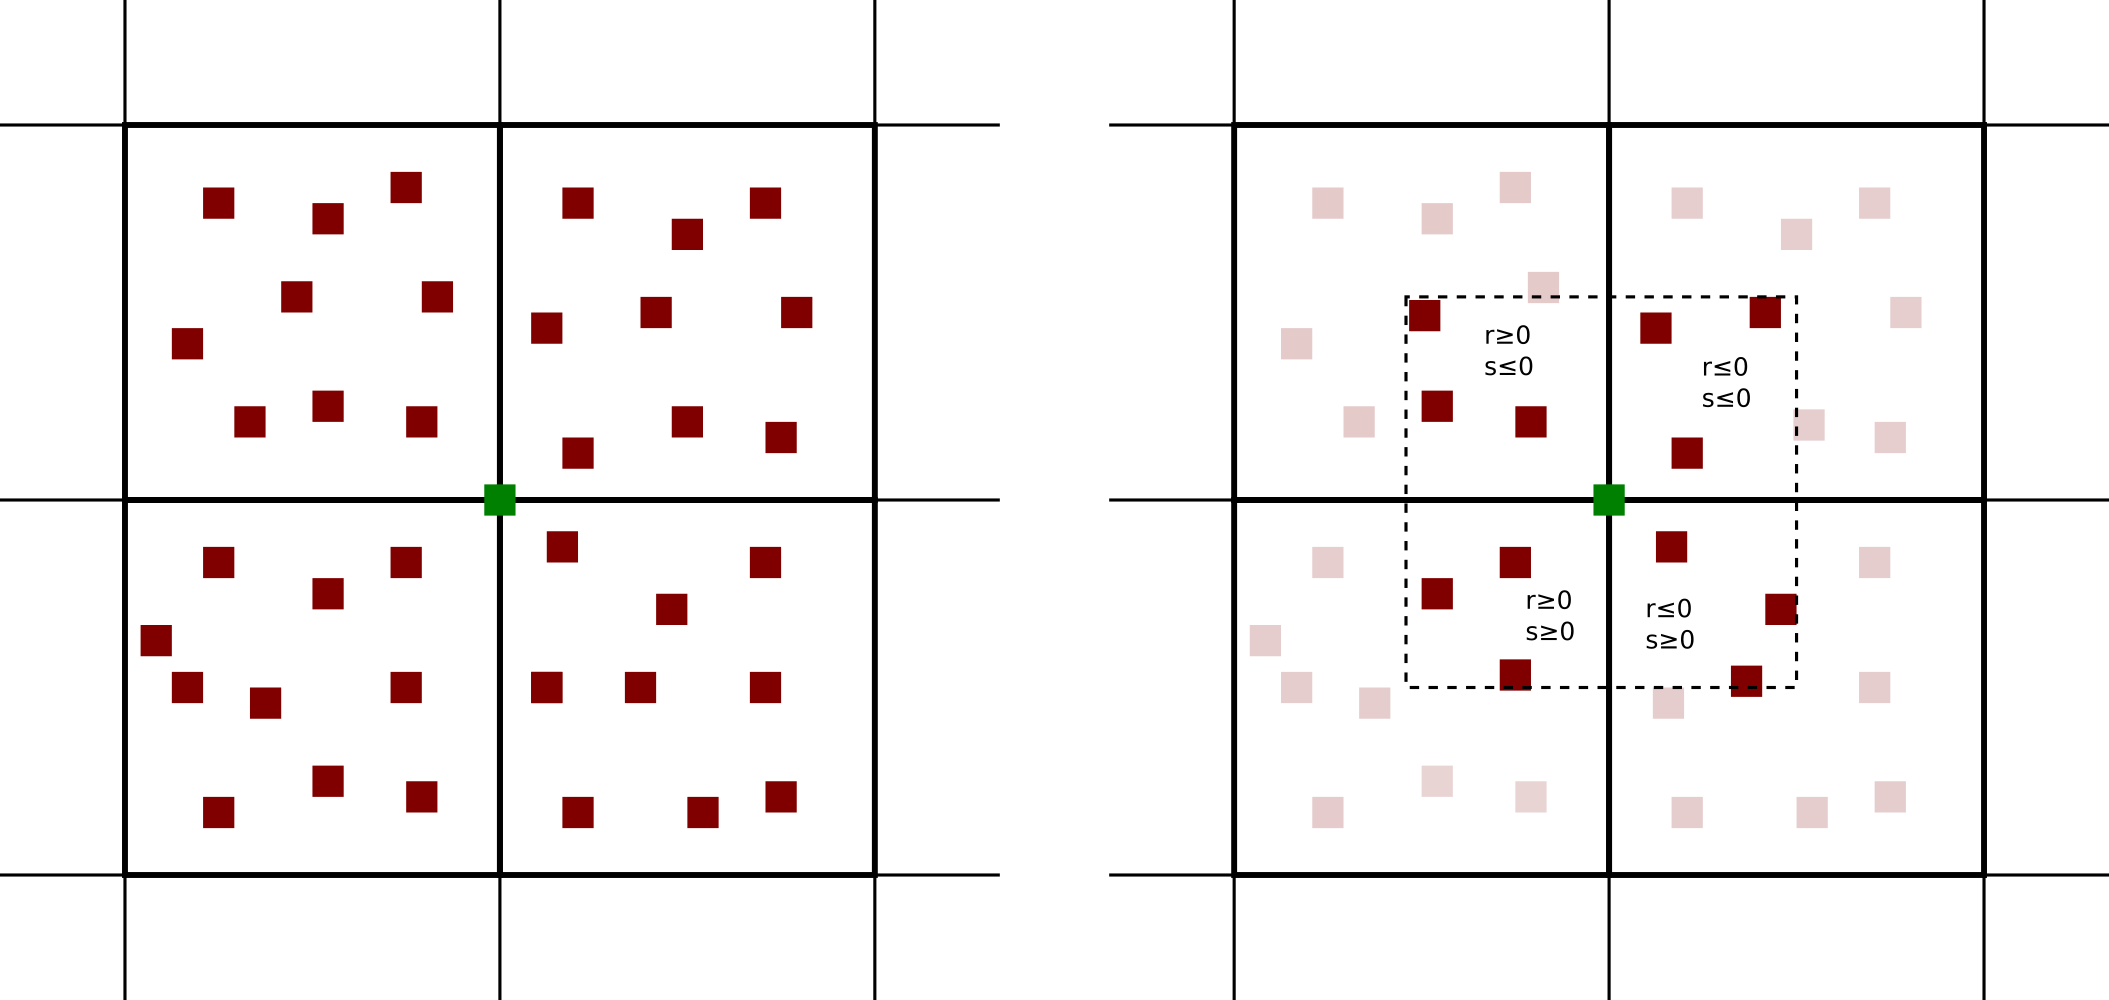
\includegraphics[width=8cm]{python_codes/fieldstone_13/markers2}\\
{\small Nodal projection. Left: all markers inside elements to which the green node belongs to are taken into account. Right: only the markers closest to the green node count. }
\end{center}

Let $k$ be the green node of the figures above. Let $(r,s)$ denote the coordinates of a marker inside its element.
For clarity, we define the follow three nodal averaging schemes:
\begin{itemize}
\item nodal type A: 
\[
f_k = \frac{\text{sum of values carried by markers in 4 neighbour elements}}
{\text{number of markers in 4 neighbour elements}}
\]
\item nodal type B: 
\[
f_k = \frac{\text{sum of values carried by markers inside dashed line}}
{\text{number of markers in area delimited by the dashed line}}
\]
\item nodal type C 
\[
f_k = \frac{\text{sum of values carried by markers in 4 neighbour elements } * N_p(r,s)}
{\text{sum of }N_p(r,s)} 
\]
where $N_p$ is the $Q_1$ basis function corresponding to node $p$ defined on each element. Since these 
functions are 1 on node $k$ and then linearly decrease and become zero on the neighbouring nodes, this
effectively gives more weight to those markers closest to node $k$.

This strategy is adopted in May et al (2014,2015) \cite{mabl14,mabl15} 
(although it is used to interpolate onto the nodes of $Q_2P_{-1}$ elements). 
It is formulated as follows:\\
"We assume that an arbitrary material point property $f$, is discretized via 
$f(\bm x)\simeq \delta(\bm x - \bm x_p) f_p$. We then utilize an approximate local $L_2$ projection
of $f_p$ onto a continuous $Q_1$ finite element space. The corner vertices of
each $Q_2$ finite element define the mesh $f_p$ is projected onto.
The local reconstruction for a node i is defined by
\[
\hat{f}_i = \frac{\int_{\Omega_i}N_i(\bm x) f(\bm x)}{\int_{\Omega_i} N_i(\bm x)} \simeq
\frac{\sum_p N_i(\bm x_p) f_p }{\sum_p N_i(\bm x_p)}
\]
where the summation over $p$ includes all material points 
contained within the support $\Omega_i$ of the trilinear interpolant $N_i$".
\end{itemize}


The setup is identical to the Stokes sphere experiment. The bash script {\sl script\_runall} 
runs the code for many resolutions, both initial marker distribution and all four 
averaging types. The viscosity of the sphere has been 
set to $10^3$ while the viscosity of the surrounding fluid is 1. 
The average density is always computed with an arithmetic mean. 




Conclusions:
\begin{itemize}
\item
With increasing resolution ($h\rightarrow 0$) vrms values seem to converge towards a single value, irrespective 
of the number of markers. 

\item
At low resolution, say 32x32 (i.e. h=0.03125), vrms values for the three averagings differ by about 10\%. At higher resolution, say 128x128, vrms values are still not converged.  

\item
The number of markers per element plays a role at low resolution, but less and less with increasing resolution. 

\item
Results for random and regular marker distributions are not identical but follow a similar trend and seem to converge to 
the same value.

\item  elemental values yield better results (espcecially at low resolutions)

\item harmonic mean yields overal the best results
\end{itemize}

\newpage
Root mean square velocity results are shown hereunder:
\begin{center}
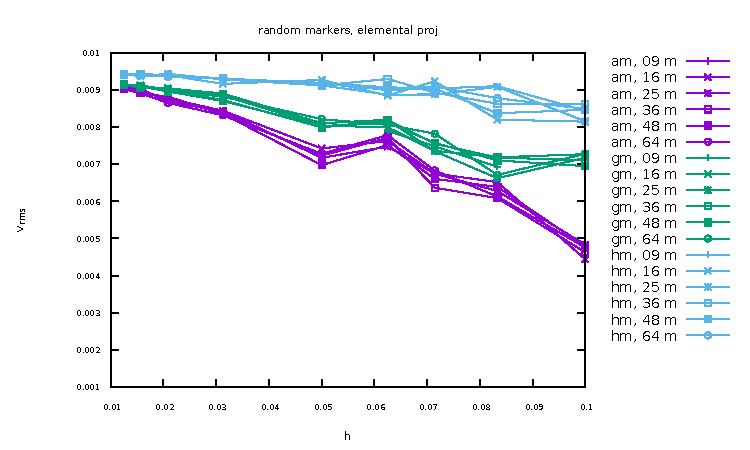
\includegraphics[width=5cm]{python_codes/fieldstone_13/vrms_rand_proj1} 
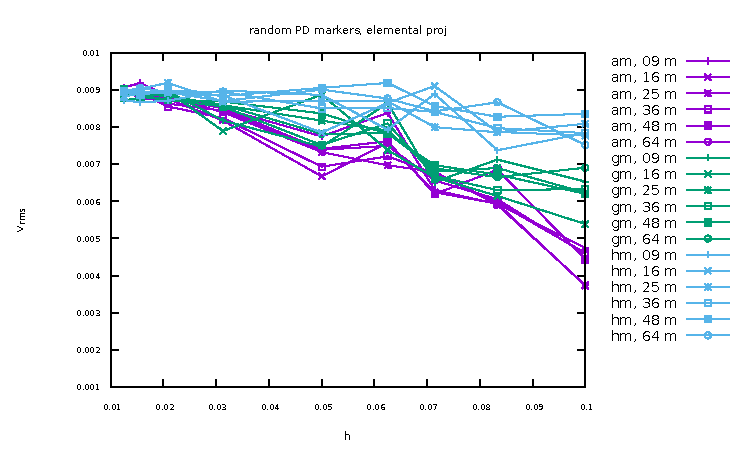
\includegraphics[width=5cm]{python_codes/fieldstone_13/vrms_poissondisc_proj1} 
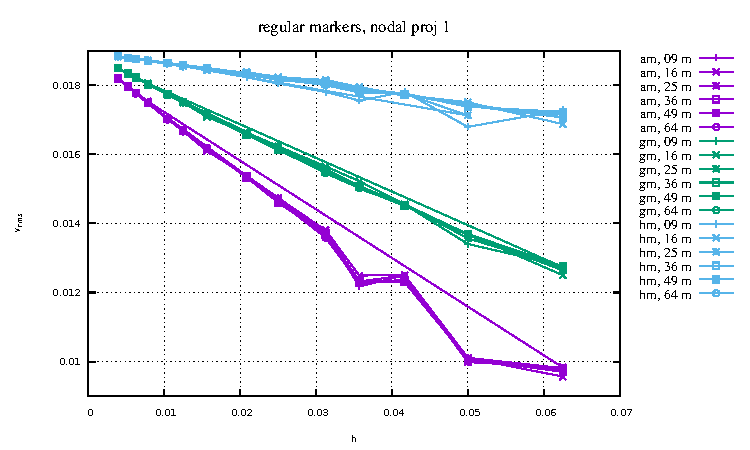
\includegraphics[width=5cm]{python_codes/fieldstone_13/vrms_reg_proj1}\\ 
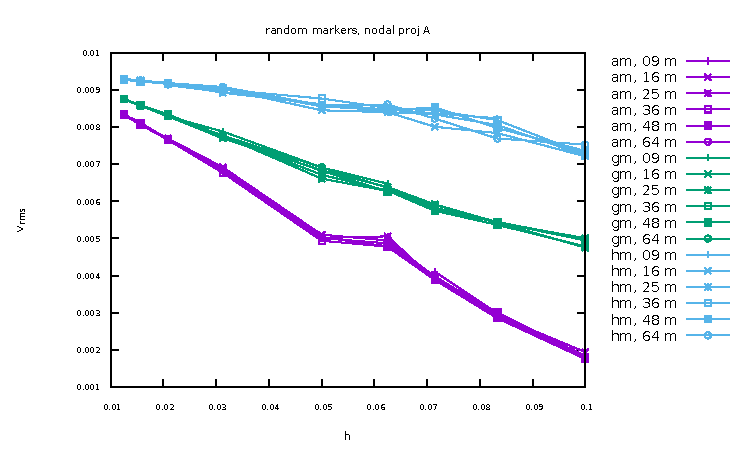
\includegraphics[width=5cm]{python_codes/fieldstone_13/vrms_rand_proj2} 
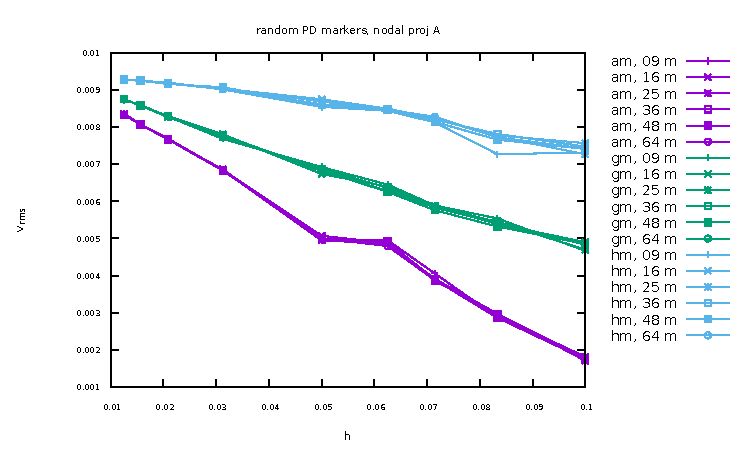
\includegraphics[width=5cm]{python_codes/fieldstone_13/vrms_poissondisc_proj2} 
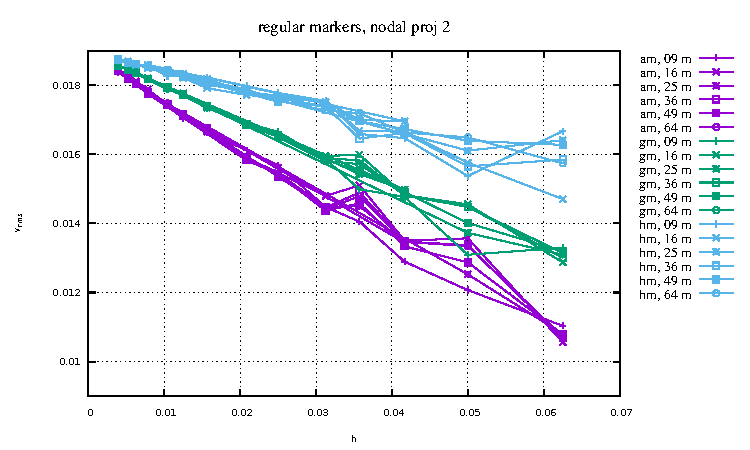
\includegraphics[width=5cm]{python_codes/fieldstone_13/vrms_reg_proj2}\\ 
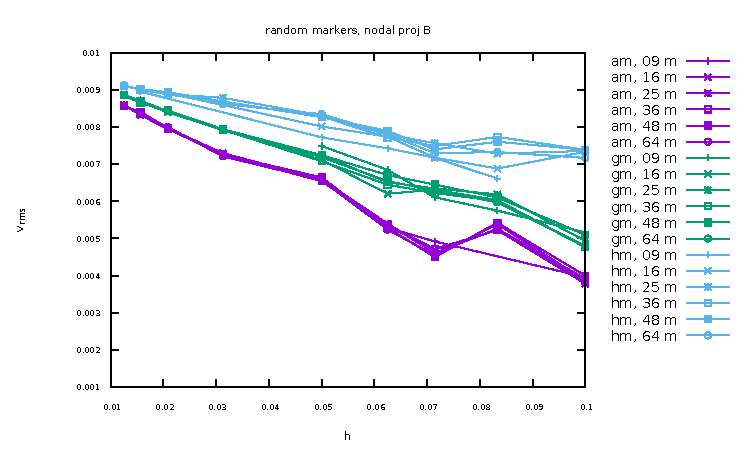
\includegraphics[width=5cm]{python_codes/fieldstone_13/vrms_rand_proj3} 
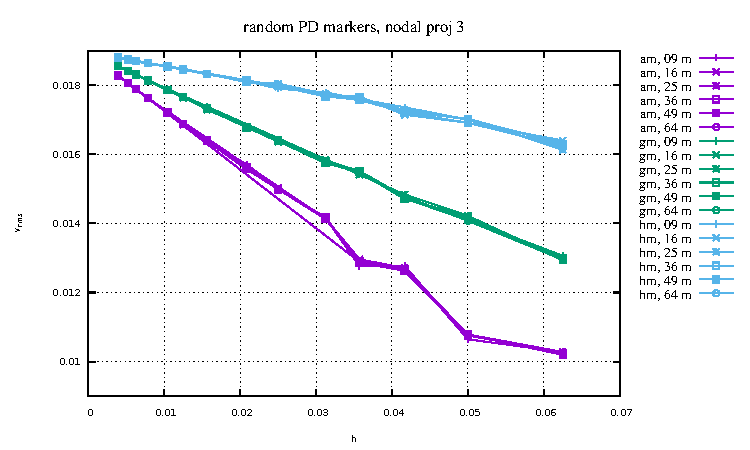
\includegraphics[width=5cm]{python_codes/fieldstone_13/vrms_poissondisc_proj3} 
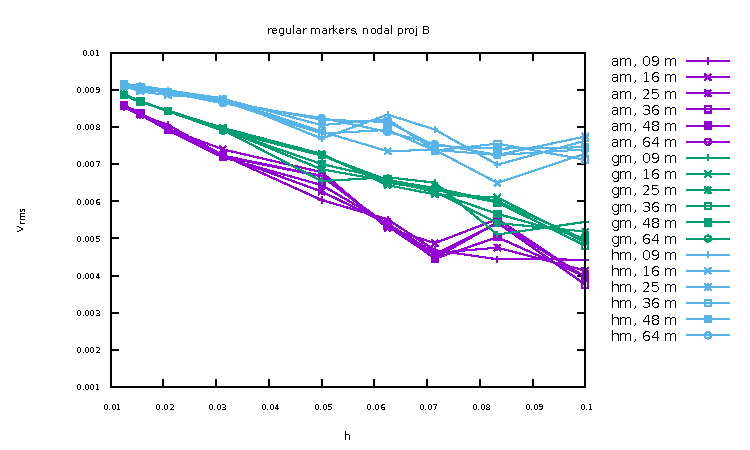
\includegraphics[width=5cm]{python_codes/fieldstone_13/vrms_reg_proj3}\\
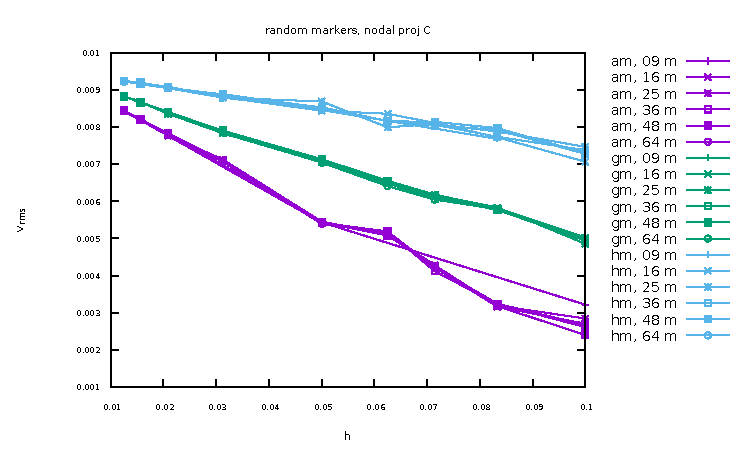
\includegraphics[width=5cm]{python_codes/fieldstone_13/vrms_rand_proj4} 
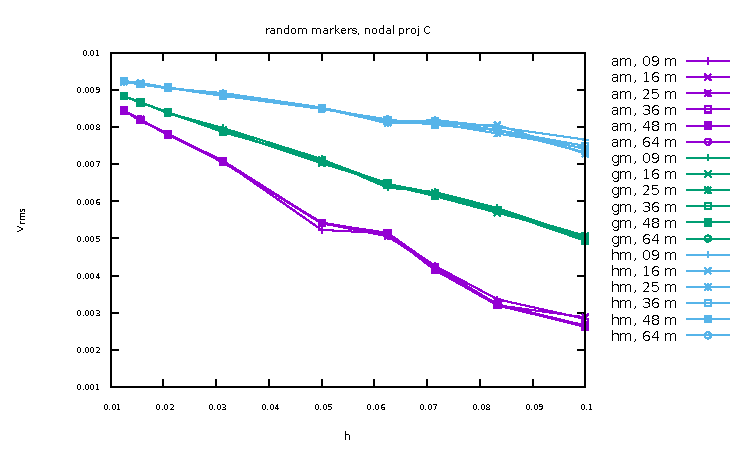
\includegraphics[width=5cm]{python_codes/fieldstone_13/vrms_poissondisc_proj4} 
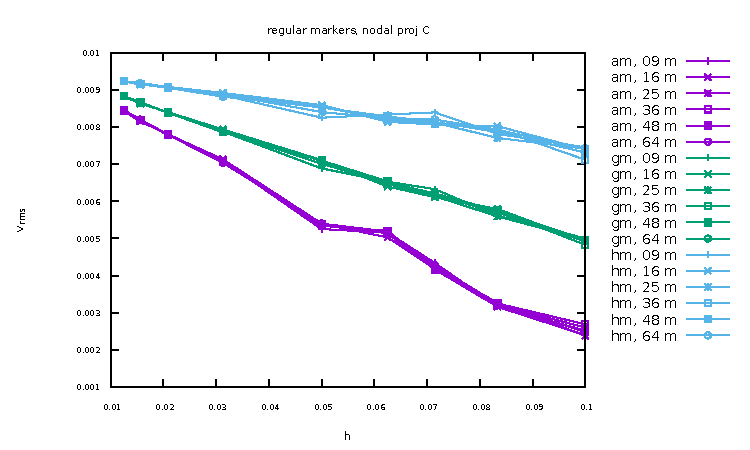
\includegraphics[width=5cm]{python_codes/fieldstone_13/vrms_reg_proj4}\\
{\small Left column: random markers, middle column: Poisson disc, right column: regular markers.
First row: elemental projection, second row: nodal 1 projection, 
third row: nodal 2 projection, fourth row: nodal 3 projection. }
\end{center}

\begin{center}
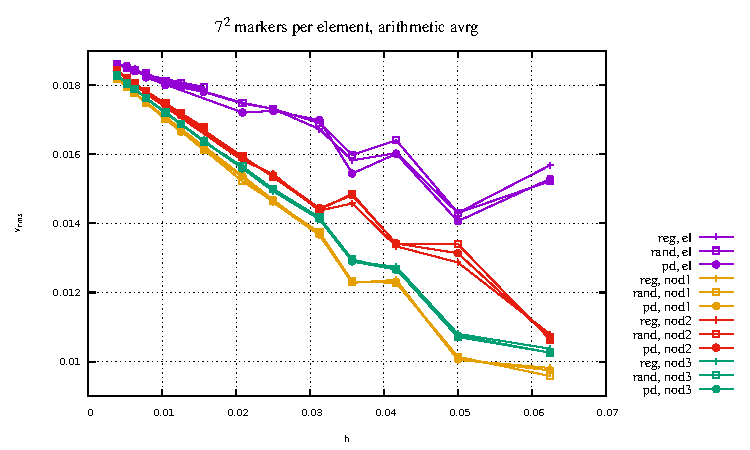
\includegraphics[width=5.cm]{python_codes/fieldstone_13/vrms_am} 
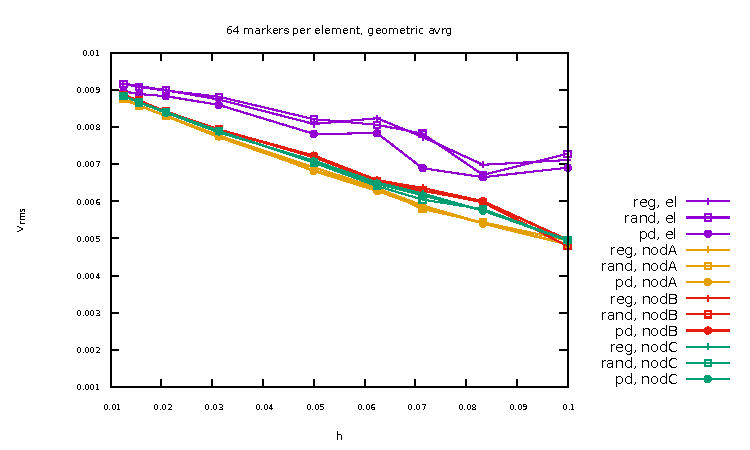
\includegraphics[width=5.cm]{python_codes/fieldstone_13/vrms_gm} 
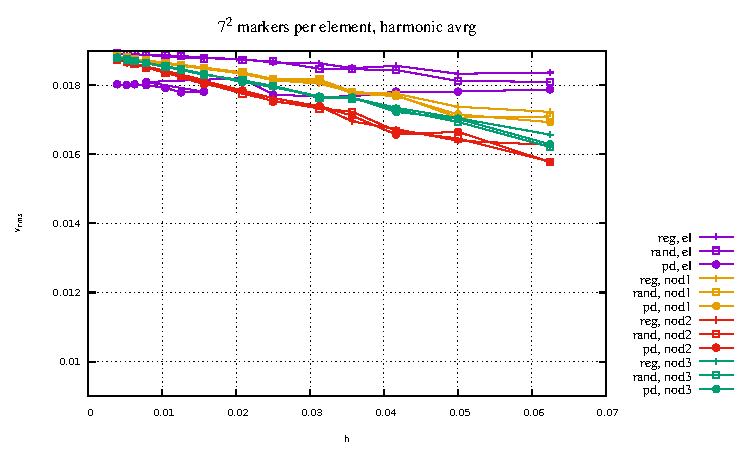
\includegraphics[width=5.cm]{python_codes/fieldstone_13/vrms_hm}\\
{\small Left to right: arithmetic, geometric, harmonic averaging for viscosity.}
\end{center}
